%%%%%%%%%%%%%%%%%%%%% chapter2.tex %%%%%%%%%%%%%%%%%%%%%%%%%%%%%%%%%
%
%  
%
% Use this file as a template for your own input.
%
%%%%%%%%%%%%%%%%%%%%%%%% Springer-Verlag %%%%%%%%%%%%%%%%%%%%%%%%%%
%\motto{Use the template \emph{chapter.tex} to style the various elements of your chapter content.}










\chapter{Constant Depth Circuit Lower Bounds}
\label{hastad} % Always give a unique label
% use \chaptermark{}
% to alter or adjust the chapter heading in the running head

%\section{Defining constant depth circuits}

Recall \Cref{def:boolean-circuit} of Boolean circuits.
We define the \emph{\textbf{depth}} of a Boolean circuit $C$ as 
the maximal length (i.e., number of edges) in a path from 
a leaf to the output node.

Here is an example of a circuit of depth 3:
\begin{figure}
    \centering
    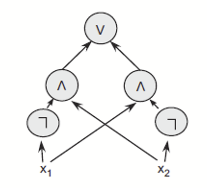
\includegraphics[width=0.2\linewidth]{images/depth_3_circuit.png}
    \label{xxx}
\end{figure}

\newcommand{\complexityclass}[1]{\sf{#1}}
\newcommand{\ACZ}{\ensuremath{\complexityclass{AC}^0}}


Recall that we are interested in the  study of the asymptotic size of circuit families, not a single circuit. That is, we want to consider how circuit size grows when the number of inputs $n$ grows. In this chapter we shall focus on circuit families $\{C_n\}_{n=1}^\infty$
whose number of inputs bits $n$ grows, their size $|C_n|$ grows polynomially while their depth is \emph{fixed} throughout the family, namly is a constant $c$ independent of $n$. 

%The class of Boolean functions computed by such circuit families is denoted $\ACZ$, and the class of such constant depth cir

%We can consider circuits of constant depth. This means that the depth of the circuit is \emph{independent of the number of inputs} $n$. In other words,  while $n$ the number of input gates can grow to infinity in the Boolean circuit family $\{C_n\}_{n=1}^\infty$, the depth of each circuit $C_n$ stays the same!


\begin{note}
If the depth of the circuit is constant and the fan-in of gates is at most two, then the number of functions we can compute with such constant-depth circuits is constant. For example, the number of variables (appearing as leaves, i.e., input nodes) is constant that way, so for a large enough number of inputs $n$, we will not be able to compute functions that read all the $n$ inputs. This means that the model is \emph{not  complete}: for a constant $d$, a depth-$d$ circuit cannot compute all Boolean functions over $n$ inputs for every $n \in \mathbb{N}$.
\end{note}

To solve this problem and make the model of constant-depth
circuits meaningful we allow \textbf{\textit{unbounded} \emph{fan-in}} gates: unbounded fan-in AND gates: $\left(\varphi_1 \wedge \varphi_2 \wedge \ldots \wedge \varphi_\ell\right)$, and unbounded fan-in OR gates
$\left(\varphi_1\lor \cdots \lor \varphi_{\ell}\right)$, where the $\varphi_i$'s are circuits (of constant depth) by themselves, with possibly \emph{joint} nodes. 
\begin{figure}
    \centering
    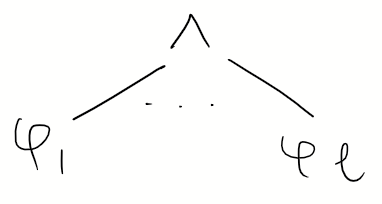
\includegraphics[width=0.2\linewidth]{images/AND.png}
    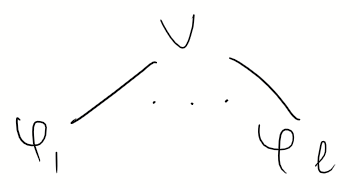
\includegraphics[width=0.25\linewidth]{images/OR.png}
    \caption{Illustration of unbounded fan-in AND and OR gates.}
\end{figure}



\newcommand{\depth}{\ensuremath{{\rm depth}}}

\begin{definition}[Depth-$d$ circuit family, constant-depth family]
\label{def:constant-depth-circuit}
A circuit family 
$\left\{\mathrm{C}_n\right\}_{n=1}^\infty$ with unbounded fan-in $\land,\lor$ gates and fan-in one negation gate is said to be of \emph{depth-$d$}, if the depth of $C_{n}$ is $d$, for all $n\in\N$. We denote by $\depth(C_n)$ the depth of the circuit $C_n$.
If $d$ is a constant (independent of $n$) we call $\left\{C_n\right\}_{n=1}^\infty$ a \emph{constant-depth family of circuits}.
\end{definition}

\textbf{Notation}: \ACZ\ denotes the complexity class 
consisting of all the functions $f:\{0,1\}^* \rightarrow\{0,1\}$ computable by  constant-depth circuit families  (equivalently, all decision problem decidable by \ACZ\ circuit families).

\para{Alternating Formulas}


We are going to use the following ``normal-form'' for constant-depth circuits. This is done for the sake of simplicity, and does not change the size of the circuits significantly, as we remark below.


A Boolean circuit is said to be an \emph{alternating  formula} if it is a formula (i.e., the underlying circuit graph is a tree), and every OR gate is followed by an AND gate followed by an OR gate, etc. Moreover, all negations in an alternating formula are pushed to the bottom of the circuit: that is, a negation node can only be connected to an input node (and that input node is not connected to any other node except a negation node). 
Here is an illustration:
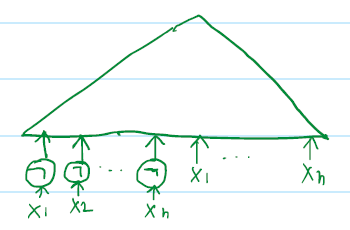
\includegraphics[width=0.3\textwidth]{image004.png}

We shall assume that all \ACZ\ circuits are alternating formulas:

% Always give a unique label
% and use \ref{<label>} for cross-references
% and \cite{<label>} for bibliographic references
% use \sectionmark{}
% to alter or adjust the section heading in the running head

\begin{svgraybox}
\textbf{Important:} From now on, when speaking about constant-depth circuits, we assume by default the fan-in of $\lor, \land$ is \emph{unbounded} ($\neg$ has fan-in one), and the circuits are \emph{alternating formulas}. 
\end{svgraybox}

\begin{exercise}
Show that every depth-$d$ circuit can be transformed into an alternating formula of depth-$O(d)$ circuit and with all negation gates on the leaves, with a polynomial size increase only.

\noindent---

\noindent{\small Hint: we can "unwind" the circuit into a formula (a tree; that is, if we used a subcircuit more than once [namely, it has out-degree more than 1], we copy this subcircuit for each such usage). Because the depth is constant this will increase the size of the circuit by at most a polynomial (exponential in a constant---i.e., polynomial). To make the formula alternating, first push all the negation to the bottom, using \emph{de Morgan rules}. And then, add dummy edges and gates to make every path from leaf to the output gate alternating between OR and AND. These all incur a polynomial increase in size.
}
\end{exercise}

\newcommand{\Parity}{\ensuremath{\operatorname{PARITY}}}

\section{Lower Bounds Against Constant-Depth Circuits for PARITY}

The function PARITY determines the parity of the total number of ones in the input bits:

\begin{tcolorbox}[colframe=white, colback=gray!11, boxrule=0mm, sharp corners]
$
\Parity(x_1,\dots,x_n): =
\begin{cases} 
1 & \text{if the number of 1's in } (x_1, x_2, \dots, x_n) \text{ is odd}, \\
0 & \text{if the number of 1's in } (x_1, x_2, \dots, x_n) \text{ is even}.
\end{cases}
$
\end{tcolorbox}

Equivalently, $\Parity$ is defined as the XOR of the input bits, denoted $x_1\parity\cdots\parity x_n$. Another equivalent definition is using modulus: $x_1+\cdots+x_n = 1 \mod 2$.

We denote by $\Parity_n$ the \Parity\ function restricted to inputs of length precisely $n$.

The main result in this chapter is the following:

\begin{theorem}[\ACZ\ lower bound for \Parity]
\label{thm:ACZ-lower bound}
Every circuit family of depth-$d$ computing the $\Parity_n$ function requires size $2^{\Omega\left(n^{\nicefrac{1}{d+1}}\right)}$.
\end{theorem}


Note: this means that if $d$ is constant, then the size lower bound is exponential: $2^{\Omega\left(n^{\nicefrac{1}{d+1}}\right)}=
2^{\Omega\left(n^k\right)}$, for some constant $0<k<1$.

The theorem is a consequence of the fact that every function in \ACZ\ can be reduced to a constant function by setting relatively few variables to constants.
The proof uses the Random Restriction Method.

\subsection{The Skeleton of the Argument: Random Restrictions}

\textbf{Upshot of argument}: The idea is to randomly restrict (assign) the variables of the circuit (of which we want to show it cannot compute \Parity). If the circuit is small, such restriction collapses (gradually) the depth of the circuit to a depth-2 circuit. If the depth of the initial circuit was constant, this gradual step-by-step depth reduction needs to be done only for a constant many times. If we made random assignments (restrictions) only for a constant many times, we can rest assure that we have not assigned (i.e., fixed) too many variables. Hence, the function $\Parity$ under these restrictions still has a lot of free variables. But such $\Parity$ with sufficiently many free variables cannot have small depth 2 circuits (this we show by an auxiliary elementary argument).
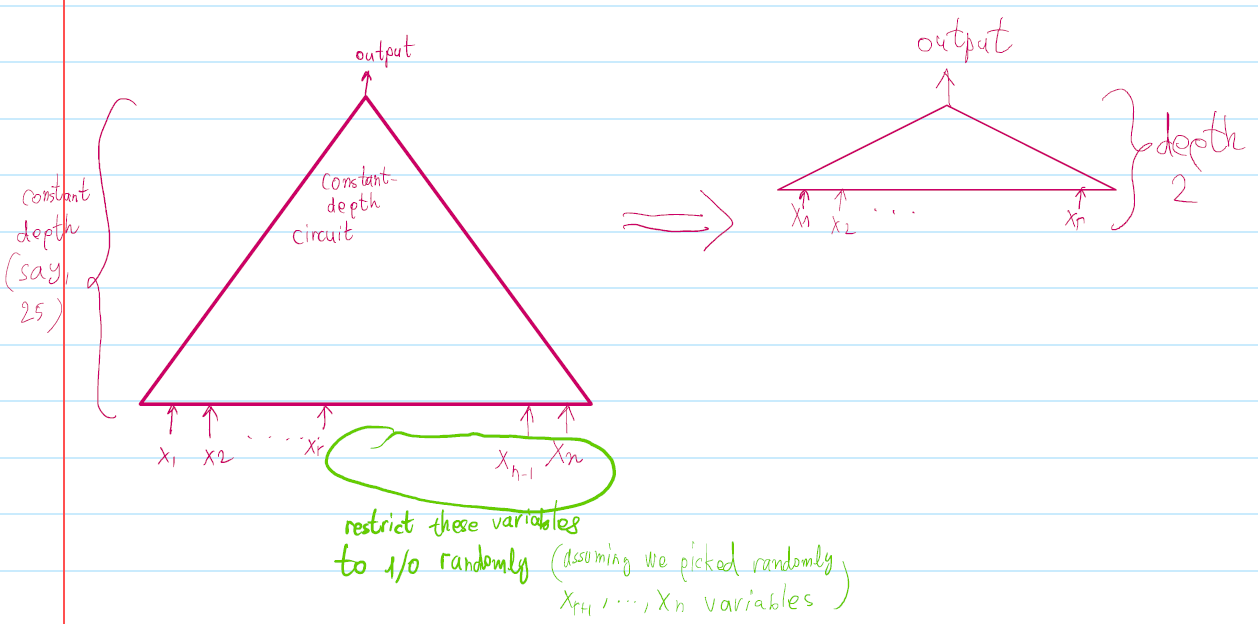
\includegraphics[width=0.9\textwidth]{image007.png}


Note the similarity with the monotone circuit lower bound proof: we use structural induction on the circuit purported to correctly compute \Parity. 

Here are the main steps of the argument in slightly more detail.

\para{Random Restriction Method}

\begin{enumerate}
\item By  way of contradiction, start with a purported small depth-$d$ circuit $C$ for $\Parity_n$.
We are going to assign to the circuit $C$ as well as to the function $\Parity_n$ it is supposed to compute random 0,1 values, showing the results of these assignments leads to conflicting effects: while the circuit restricted to these assignments becomes a circuit that computes a very simple function with high probability, the function $\Parity_n$ is still a rather complicated function to compute even after all this restriction, with high probability.
\item Let $\overline x$ be $n$ variables $x_1,\dots,x_n$. Pick a random assignment $\rho_0: \overline x \rightarrow\{0,1, *\}^n$ with ``$x_i \rightarrow *$'' meaning that $x_i$ is \emph{un-assigned}, namely, stays a \emph{free} variable. We make sure that enough $x_i$'s stay  free.

\item Depth Reduction Step: 
%\item   $f$ is resilient in the sense that $f\rst\rho
%%\not\equiv 0$;

If $C$ is a small circuit then the \emph{function} computed by $C\rst\rho_0$, namely the restriction of $C$ to the assignment $\rho_0$, has a depth  $d-1$ circuit of small size. 

\item
Sequentially we assign new random restrictions $\rho_1,\dots,\rho_{d-3}$
 (extending $\rho_0$) so that we reduce the depth of $C$ by 1 each time, until the depth is 2.

\item 
At this point, we end up with a circuit $C^{\prime}$ of depth 2 that computes the function 
$\Parity_n\rst\rho_0\rho_2\ldots\rho_{d-3}$.

\item
We now use an auxiliary statement to reach a contradiction: since we made sure that each assignment $\rho_i$ leaves enough variables free, $\Parity_n\rst\rho_0\rho_2\ldots\rho_{d-3}$
is still a relatively "complex" function, with high probability. In particular, we show that there are no \emph{small} depth $2$ circuits (i.e., OR of ANDs or ANDs of ORs) that compute $\Parity_n\rst\rho_0\rho_2\ldots\rho_{d-3}$.
\end{enumerate}


% \textcolor{red}{
% \begin{Huge}
% To Be Completed!\end{Huge}}



